\usepackage{titlesec} % defining font styles for sections etc

\titleformat{\section}
{\normalfont\scshape}{\thesection}{1em}{}[\vspace{2ex}\titlerule]

\titlespacing{\section}{-45pt}{10ex plus 1ex minus .2ex}{4.3ex plus .2ex}

\newcommand{\sectionbreak}{\clearpage}

\titleformat{\subsection}
{\huge\bfseries}{\small\thesubsection}{.8em}{}

\titlespacing{\subsection}{0pt}{8ex plus 1ex minus .2ex}{1ex plus .2ex}


\usepackage{array} % for defining a new column type
\usepackage{varwidth} %for the varwidth minipage environment
\usepackage{caption}
\usepackage{adjustbox}
\usepackage{longtable}
\usepackage{graphicx}
\usepackage{tabulary}
\usepackage[a4paper, total={6in, 8in}]{geometry}
\usepackage[table,dvipsnames]{xcolor}
\usepackage[
hidelinks,
colorlinks,
allcolors=black,
bookmarks=true	
]{hyperref}
\usepackage[
numbered,
open,
openlevel=1
]{bookmark}
%\usepackage[pages=all]{background}
\usepackage[firstpage=true]{background}
\backgroundsetup{
	scale=1,
	color=black,
	opacity=0.4,
	angle=0,
	contents={%
		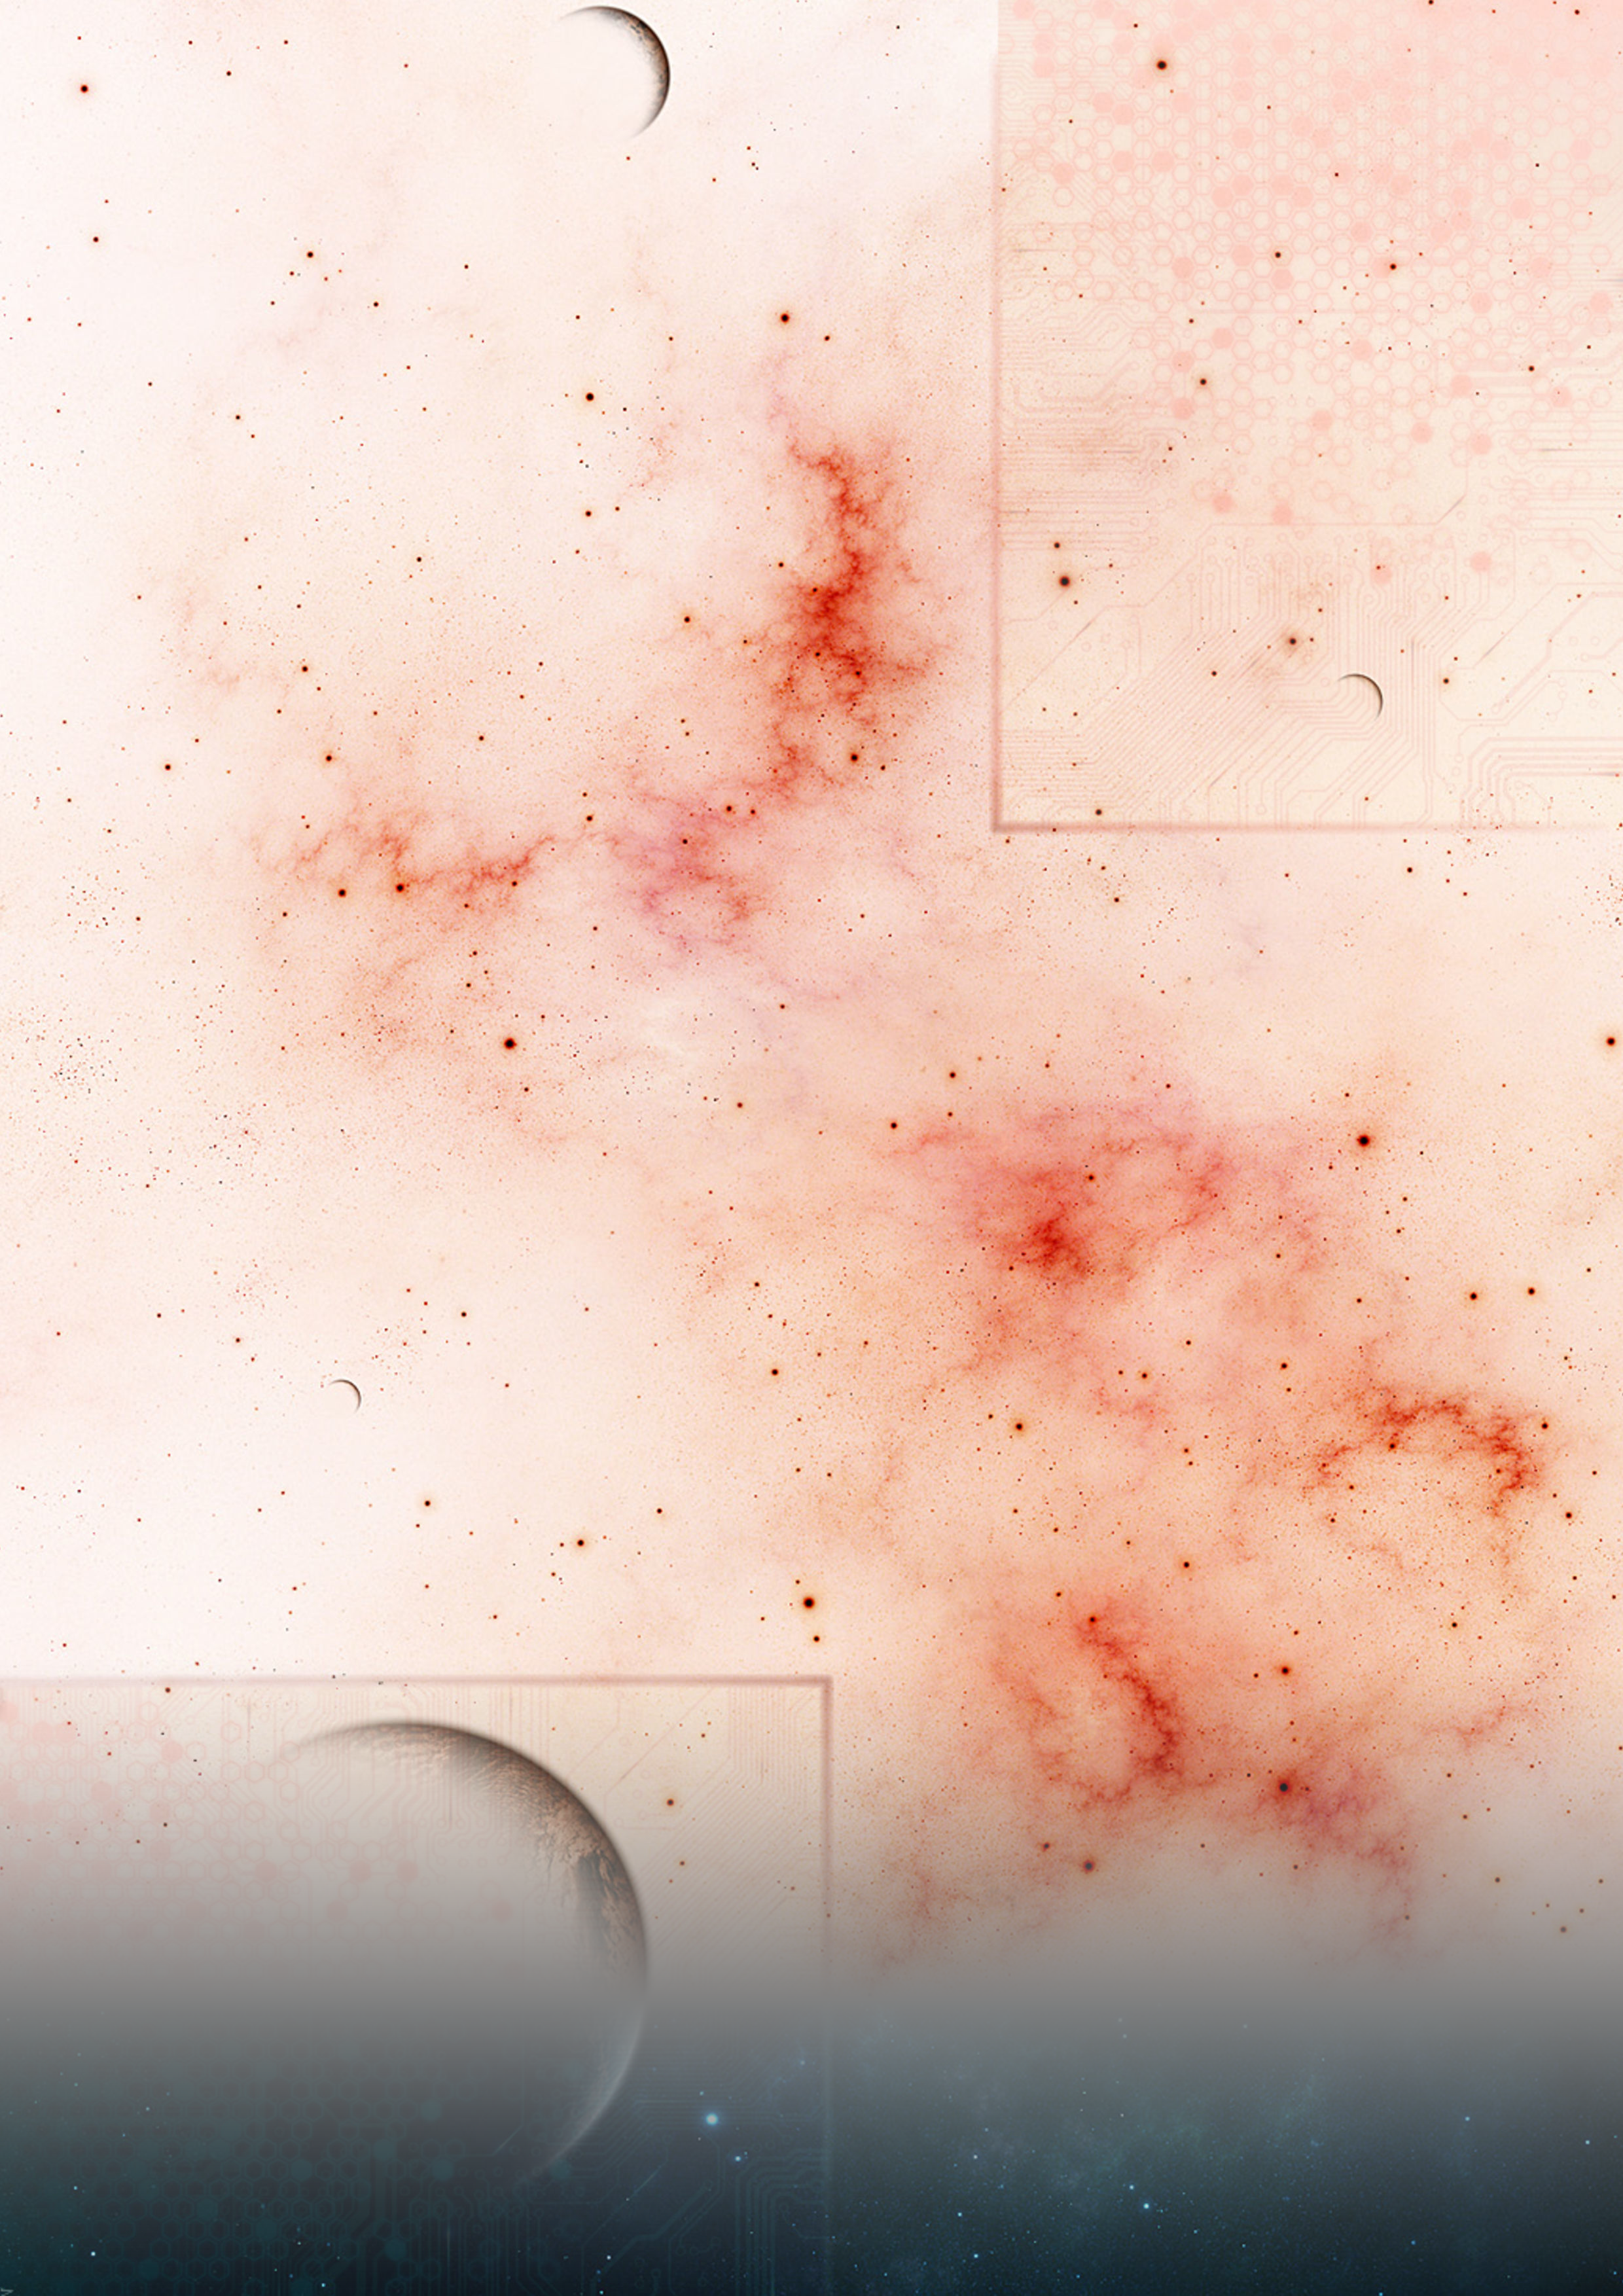
\includegraphics[width=\paperwidth,height=\paperheight]{Background2}
	}%
}

%   Schriftart der auf den Karten eingesetzten Texte
\usepackage{anttor}

%   UTF-8 Encoding der TeX-Dateien
\usepackage[utf8]{inputenc}

%   englisches Sprachpaket
\usepackage[english]{babel}

%   optischer Randausgleich
\usepackage{microtype}

\usepackage{color}

%   TikZ zum "Malen" von Grafiken, in diesem Falle für die Karten
\usepackage{tikz}
\usetikzlibrary{patterns}
\usetikzlibrary{shadows}

%   Symbole dazuladen; Verwendung \ding{<nummer>}
\usepackage{pifont}
%   weitere Symbole
\usepackage{fourier-orns}